\documentclass[class=report,crop=false, 12pt]{standalone}
\usepackage[screen,nosolutions]{../scratch}

\begin{document}

\titre[S]{Variables et hasard}
%===============================


\insertvideo{2HUEeyoJpKc}{Variables et hasard -- Activité 1}

\insertvideo{YX3yYVIsktw}{Variables et hasard -- Activité 2}

\insertvideo{e2BUoqQGkX0}{Variables et hasard -- Activité 3}

\bigskip
\bigskip


\begin{activite}
Ce jeu est un grand classique de la programmation :
\begin{itemize}
  \item L'ordinateur choisit au hasard un nombre secret entre $1$ et $50$.
  \item Le joueur propose une réponse.  
  \item L'ordinateur répond \og le nombre à trouver est plus grand \fg{} ou bien \og le nombre à trouver est plus petit \fg{} jusqu'à ce que ce que le joueur trouve la bonne réponse !
\end{itemize}

\begin{center}
  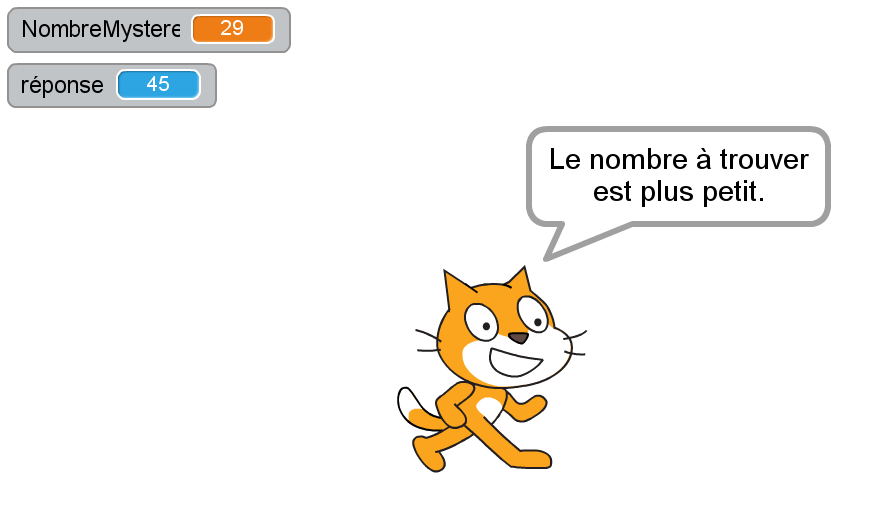
\includegraphics[scale=\scaleecran]{ecran-06-ex1} 
\end{center}


\bigskip

\textbf{Blocs utiles.}

\begin{itemize}
  \item Tu auras besoin de créer tes propres variables. Dans une variable, on peut mettre par exemple un nombre, on peut changer ce nombre au cours de l'exécution du programme et on peut utiliser la valeur contenue dans la variable n'importe où dans le programme. Voici un exemple avec la variable \og mavariable \fg{}, créée dans la catégorie \og Données \fg{} par \og Créer une variable \fg{}.
  
\begin{center}
  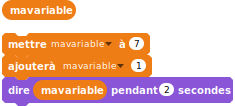
\includegraphics[scale=\scalebloc]{bloc-06-ex1a} 
\end{center} 
  
  \item Le bloc \og nombre aléatoire entre (1) et (50)\fg{} permet de tirer au hasard un nombre entier compris entre $1$ et $50$.
  

\begin{center}
  
\includegraphics[scale=\scalebloc]{bloc-06-ex1b}
\end{center}

\end{itemize}

\end{activite}




\begin{activite}

Tu vas tracer le \emph{triangle de Sierpinski}, qui est un triangle rempli de trous, en plaçant des points au hasard !

Voici seulement le début de la construction :
\begin{center}
  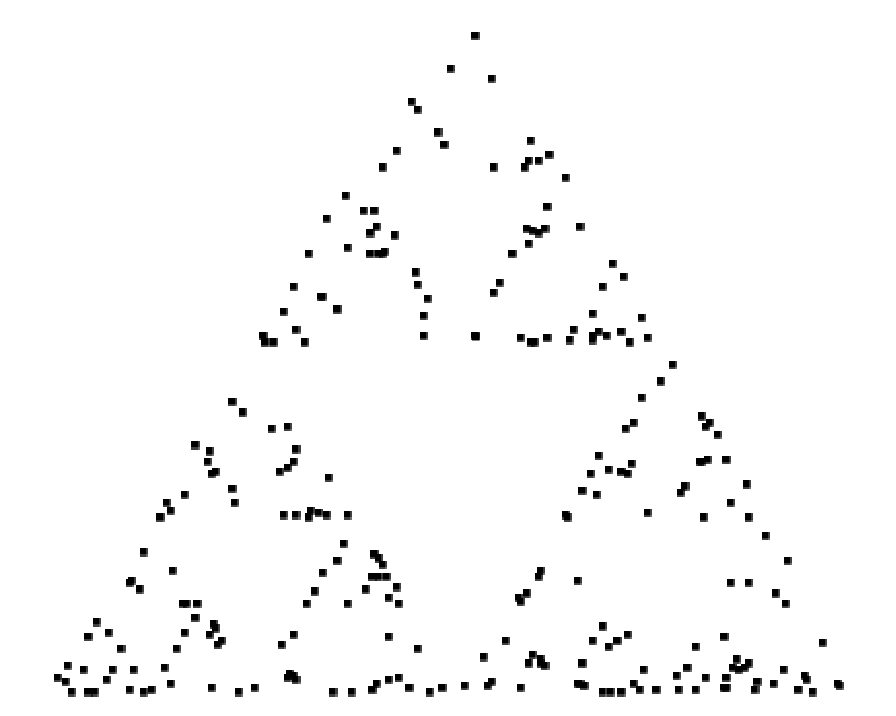
\includegraphics[scale=\scaleecran,scale=0.7]{ecran-06-ex2} 
\end{center}

Le principe du tracé est le suivant :
\begin{itemize}
  \item Je pars d'un point $P_1$.
  \item Je choisis au hasard l'un des sommets du triangle.
  \item Je trace le point $P_2$ qui est le milieu entre $P_1$ et ce sommet.
  \item Je recommence le processus en partant cette fois du point $P_2$ qui vient d'être défini...
\end{itemize}

Sur les dessins ci-dessous, on a placé $P_1$, le premier sommet choisi est $S_2$, on trace le milieu de $[P_1S_2]$, c'est $P_2$. On repart de $P_2$, le second sommet choisi est ici $S_1$ et $P_3$ est le milieu de $[P_2S_1]$. On choisit de nouveau le sommet $S_2$ afin de tracer $P_4$...

\myfigure{0.91}{
\footnotesize
\tikzinput{sierp1}\quad
\tikzinput{sierp2}\quad
\tikzinput{sierp3}\quad
\tikzinput{sierp4}
}

Voici comment programmer :
\begin{itemize}
  \item Définir deux variables $x$ et $y$, qui seront les coordonnées du point qui vient d'être tracé.
  
  \item Choisir au hasard un nombre entre $1$ et $3$.
  \begin{itemize}
    \item Le nombre $1$ correspondra au sommet $S_1$ de coordonnées $(-200,-170)$.
    \item Le nombre $2$ correspondra au sommet $S_2$ de coordonnées $(+200,-170)$.
    \item Le nombre $3$ correspondra au sommet $S_3$ de coordonnées $(0,+170)$.        
  \end{itemize}
    
  \item Si $(x,y)$ sont les coordonnées du point $P$, alors on trouve les coordonnées
  du milieu entre $P$ et $S_1$, en calculant les moyennes des coordonnées :
  $$\left(\frac{x-200}{2} ,\frac{y-170}{2}\right)$$
  
  Donc selon que l'on choisit $S_1$, $S_2$ ou $S_3$, on fait :
  $$
  \left\{\begin{array}{rcl}x &\leftarrow& \frac{x - 200}{2} \\ y &\leftarrow& \frac{y -170}{2}\end{array}\right.\qquad\qquad
  \left\{\begin{array}{rcl}x &\leftarrow& \frac{x + 200}{2} \\ y &\leftarrow& \frac{y -170}{2}\end{array}\right.\qquad\qquad
  \left\{\begin{array}{rcl}x &\leftarrow& \frac{x}{2}  \\ y &\leftarrow& \frac{y + 170}{2}\end{array}\right.
  $$
  
  \item On répète ce processus indéfiniment (le mode turbo permet d'aller plus vite).
  
  \item On trace chaque point par la commande \og estampiller \fg{} (donner un coup de tampon). On aura au préalable remplacé le dessin de Scratch par un tout petit carré noir.
\end{itemize}


\end{activite}






\begin{activite}

Tu vas programmer un petit jeu de ping-pong :
\begin{itemize}
  \item La raquette (en noir) se déplace à droite et à gauche avec les touches de flèches.
  \item La balle tombe (avec une position de départ et un angle pris au hasard).
  \item Si la balle tombe sur la raquette ou touche un mur, elle rebondit.
  \item Si la balle touche la zone rouge du bas, c'est perdu.
  \item De plus, chaque fois que la balle touche la raquette, elle accélère !
\end{itemize}

\begin{center}
  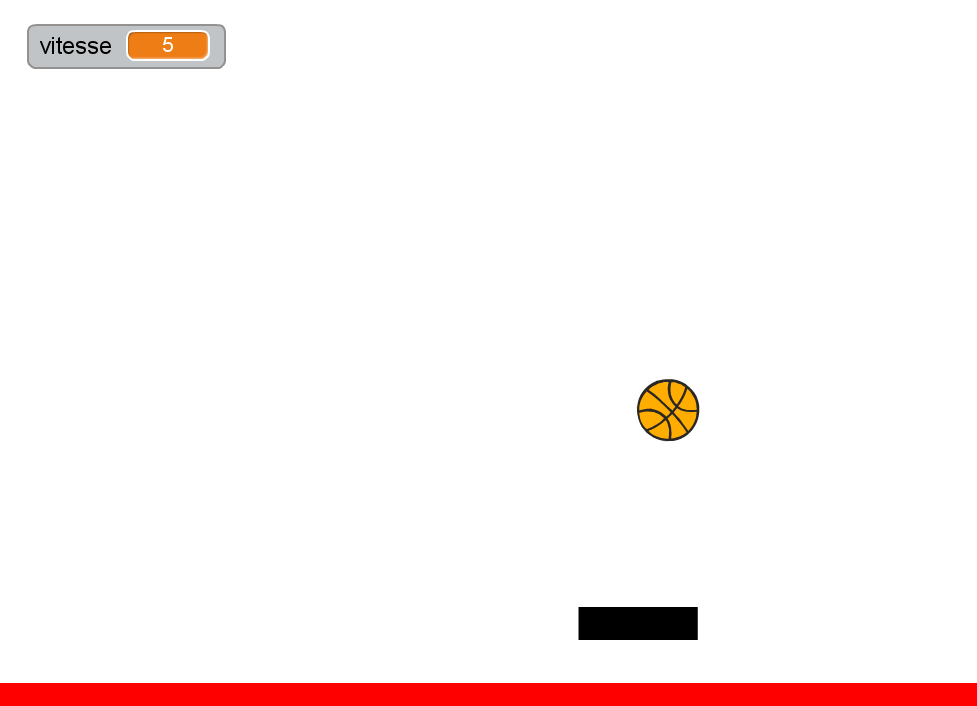
\includegraphics[scale=\scaleecran,scale=0.9]{ecran-06-ex3} 
\end{center}

\bigskip
\textbf{Arrière-plan.}

Dessine tout en bas de l'arrière-plan un rectangle rouge long et mince.

\bigskip
\textbf{La raquette.}

La raquette est le premier lutin. Remplace le chat Scratch par un petit rectangle noir.
Le programme associé à la raquette est très simple : lorsque le drapeau vert est cliqué, 
la raquette se déplace vers la droite ou vers la gauche avec les touches de flèches.

\bigskip
\textbf{La balle.}

La balle est un second lutin, qui aura son propre programme.

\begin{itemize}
  \item Lorsque le drapeau vert est cliqué, place la balle en position ($x$, 180) avec pour $x$ un nombre pris au hasard entre $-150$ et $+150$.
  \item Oriente la balle au hasard avec un angle entre $160$ et $200$.
  \item Définis une variable \og vitesse \fg{}, au départ la vitesse vaut $5$. 
  \item Répète indéfiniment :
  \begin{itemize}
    \item avancer la balle de la valeur \og vitesse \fg{},
    \item si la zone rouge est touchée, arrêter tout : c'est perdu !
    \item rebondir si le bord est atteint,  
    \item si la zone noire est touchée (la raquette) alors rebondir et augmenter la vitesse de $1$.      
  \end{itemize}
\end{itemize}

\bigskip
\textbf{Comment rebondir ?}
La balle arrive avec un certain angle. Cet angle est stocké dans la variable \og direction \fg{}.
Lorsqu'elle touche la raquette (le rectangle noir), alors la balle doit changer sa direction.
La formule est la suivante :
$$\text{nouvelle direction} = 180^\circ - \text{ancienne direction}.$$

\myfigure{0.8}{
\tikzinput{rebondir}
}

Ce qui s'écrit :
\begin{center}
  
\includegraphics[scale=\scalebloc]{bloc-06-ex3}
\end{center}

\end{activite}



\ifx \displaysolutions \myzero
\else
\begin{code}
\onesolution{Variables et hasard}{Activité 1}{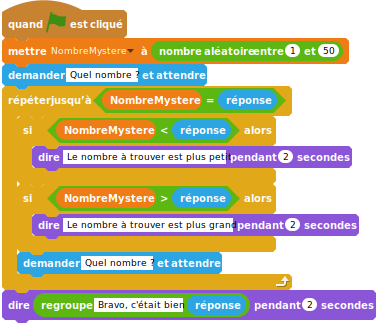
\includegraphics[scale=\scalesolution]{code-06-ex1}}
\onesolution{Variables et hasard}{Activité 2}{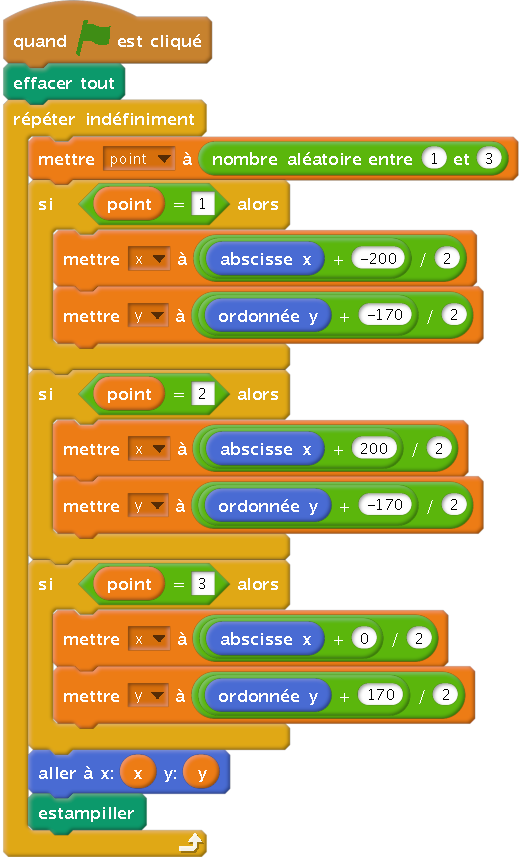
\includegraphics[scale=\scalesolution]{code-06-ex2}}
\onesolution{Variables et hasard}{Activité 3}{
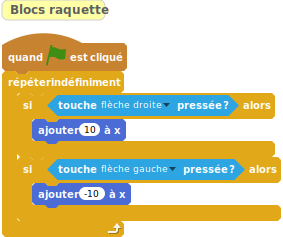
\includegraphics[scale=\scalesolution]{code-06-ex3a}
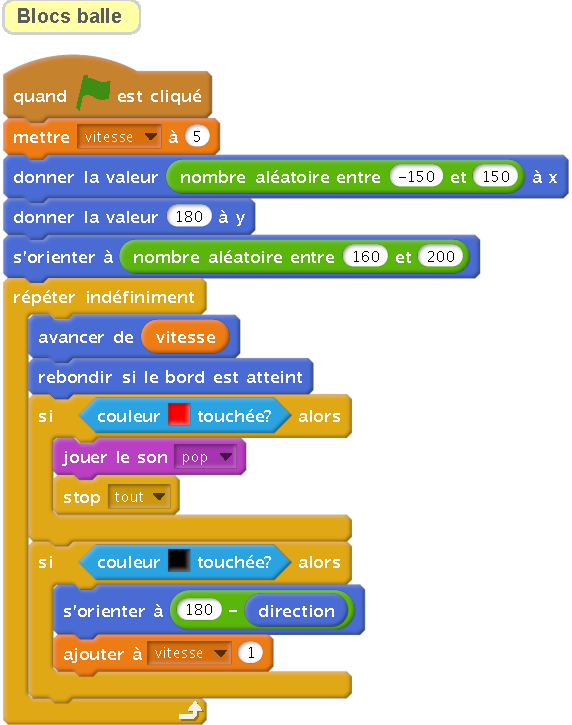
\includegraphics[scale=\scalesolution]{code-06-ex3b}
}    
\end{code}
\fi


\end{document}

